% The first argument is the \documentclass, which tells latex which template
% we're using to build this document. It's usually safe to just use "article".
\documentclass{article}

% include some packages...
\usepackage{fullpage} % change settings for a smaller margin
\usepackage{graphicx} % gives access to the \includegraphics commands
\usepackage{amsfonts}
\usepackage{float}
\usepackage{enumitem}
\usepackage{caption}
\usepackage[export]{adjustbox}
\usepackage{bookmark}
\graphicspath{{./images/}}

% tell Latex to use no paragraph indentation, but leave some space between
% paragraphs
\setlength{\parindent}{0in}
\setlength{\parskip}{0.1in}

\newcommand{\tib}[1]{\textit{\textbf{#1}}}
\newcommand{\code}[1]{\texttt{#1}}

% these commands merely set the values for the title/date/author; they don't put
% them in the document... see \maketitle below
\title{CS Department Automated Information Timeline \\ Assignment 8.2: State/Package/Deployment}
\date{\today}
\author{Matthew Hays, Pawan Bhandari, Sarah Faron, Tim Klimpel \\ The Incredibles}

% all document content goes between \begin{document} and \end{document}
\begin{document}

% this command actually creates the title/date/author in the document
\maketitle
\newpage
\tableofcontents
\listoffigures
\newpage
\section{Introduction}
\subsection{Purpose}
The purpose of this assignment is to collaborate as a team and create a state machine diagram, package diagram and a deployment diagram for the CS Department Automated Information Timeline project. Team members met multiple times over the course of few days to work together and create these diagrams which are presented in the subsequent sections.

\section{State Machine Diagram}

\begin{figure}[H]
    \centering
    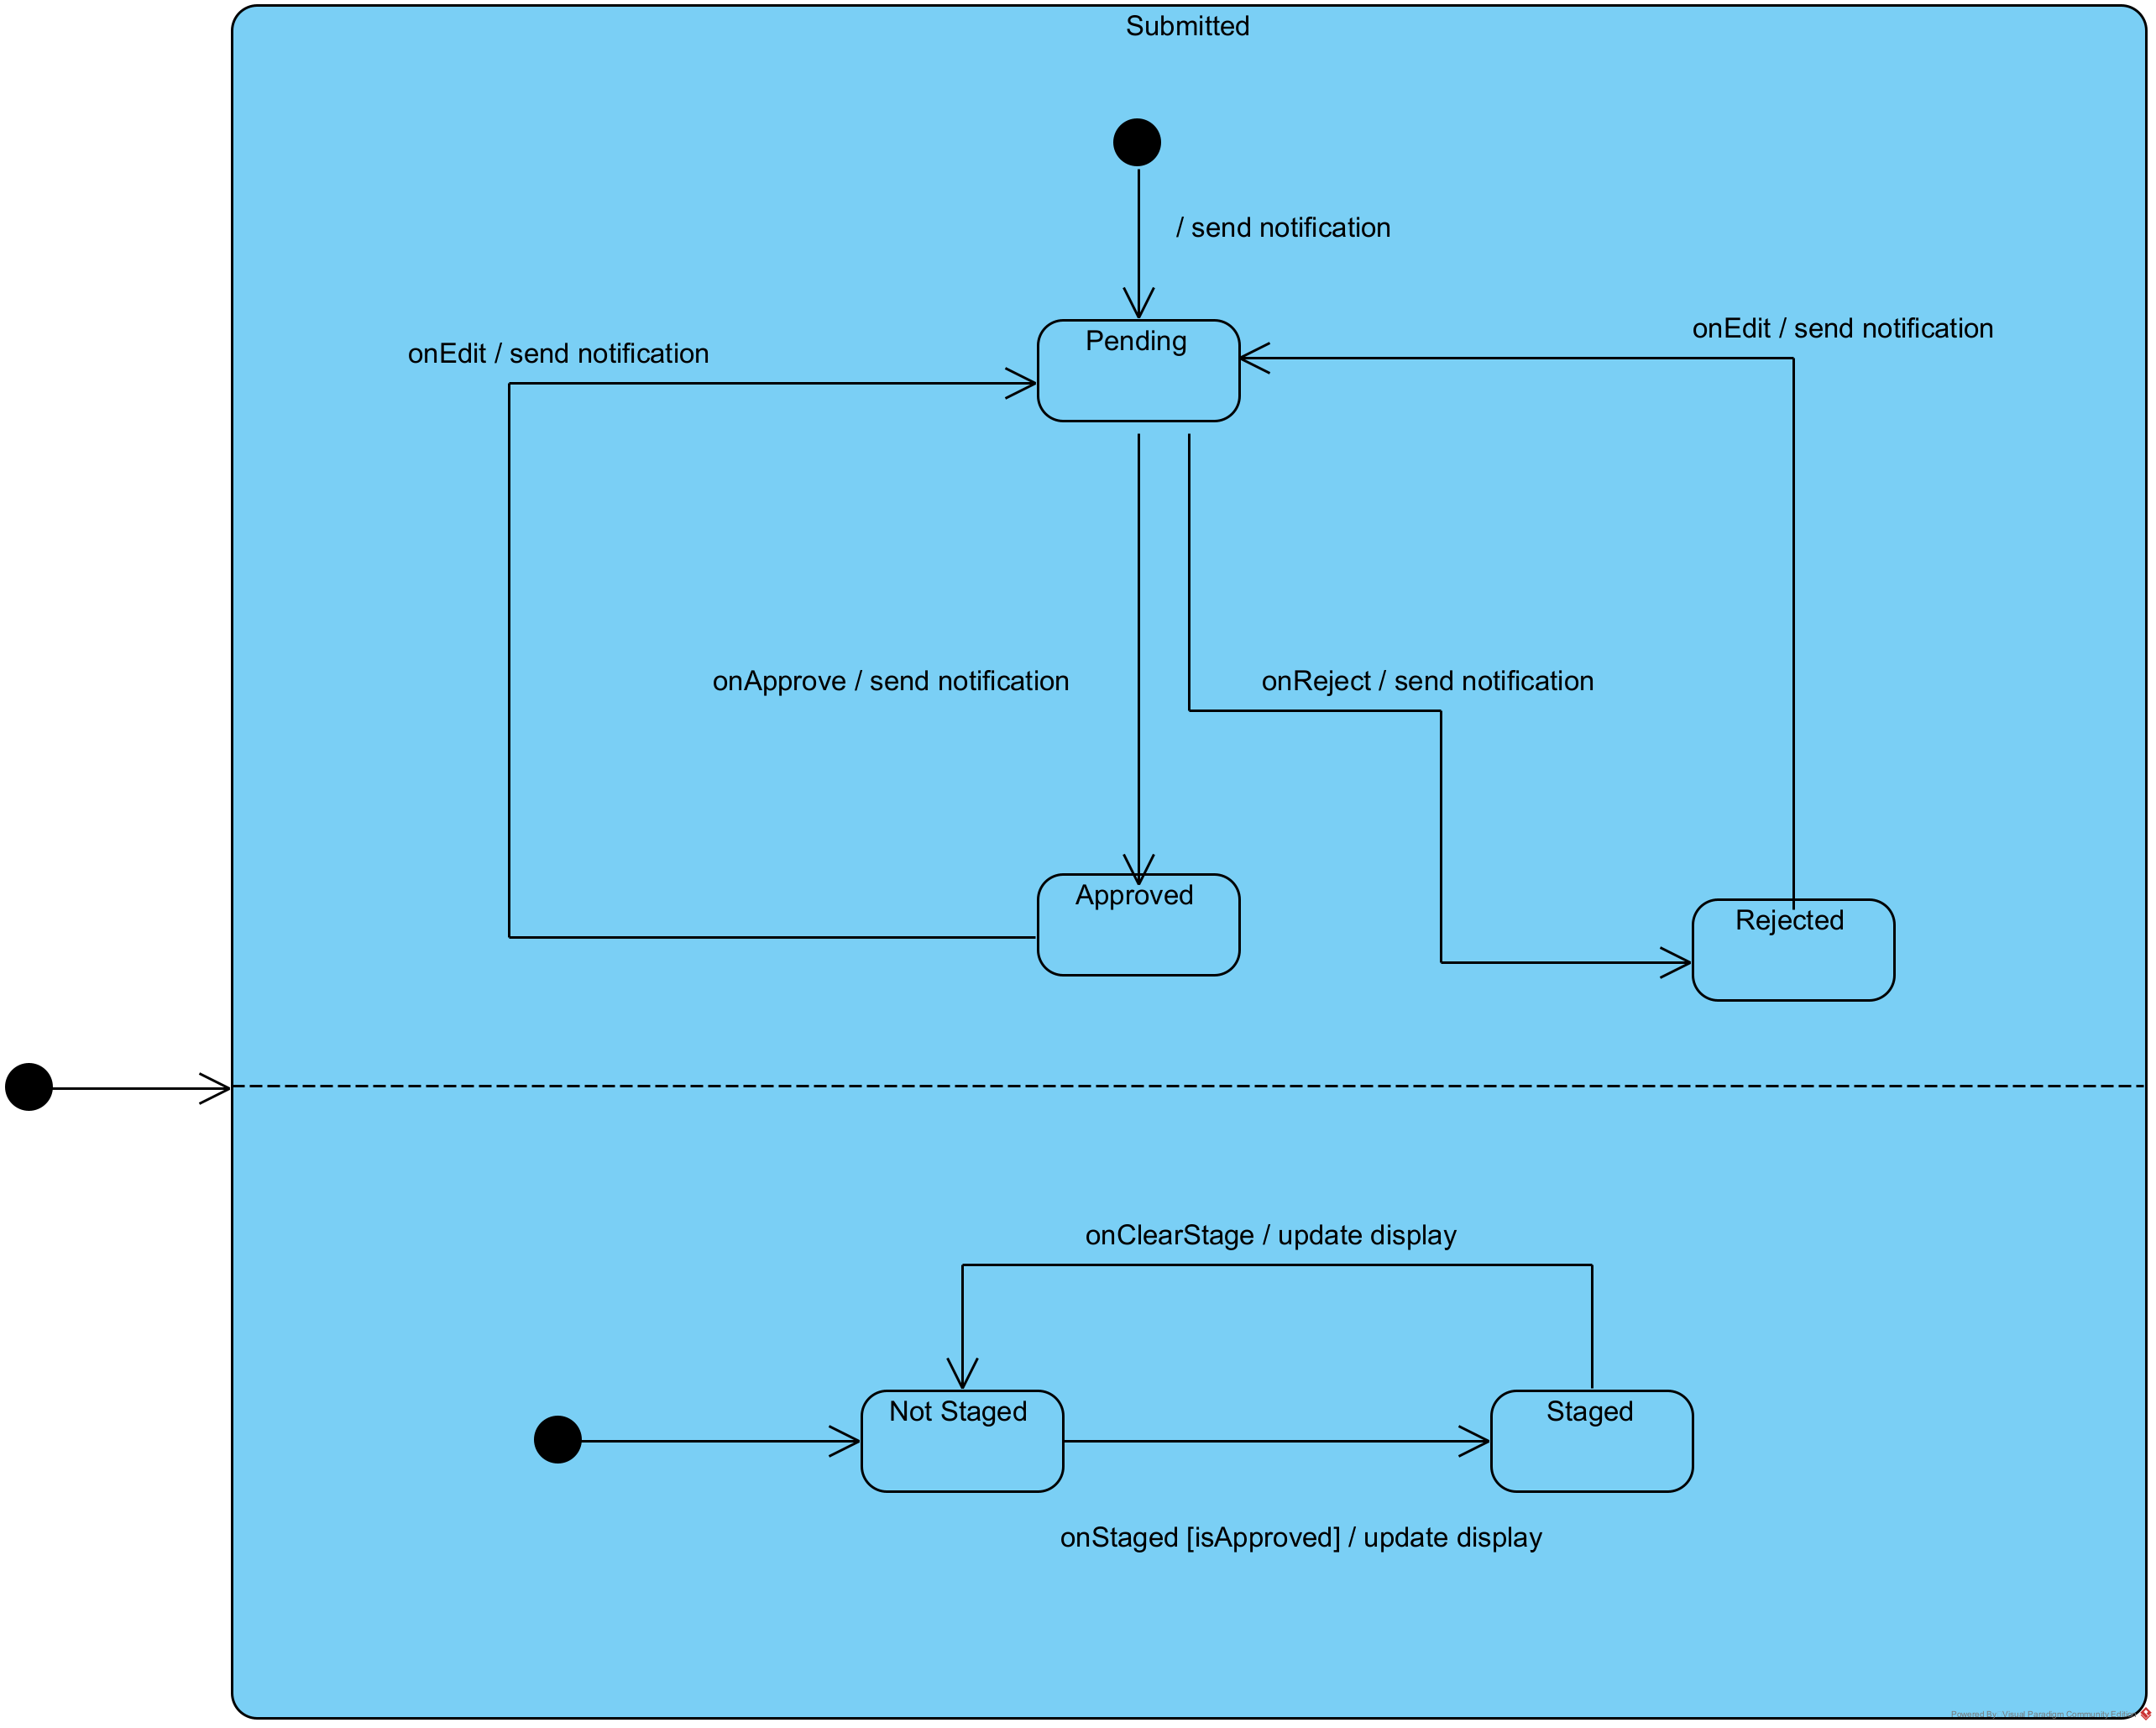
\includegraphics[width=.98\textwidth]{images/State_Machine_Diagram.png}
    \centering
    \caption{State Machine Diagram for review and staging of submitted posts, events and pages.}
\end{figure}

\section{Package Diagram}

\begin{figure}[H]
    \centering
    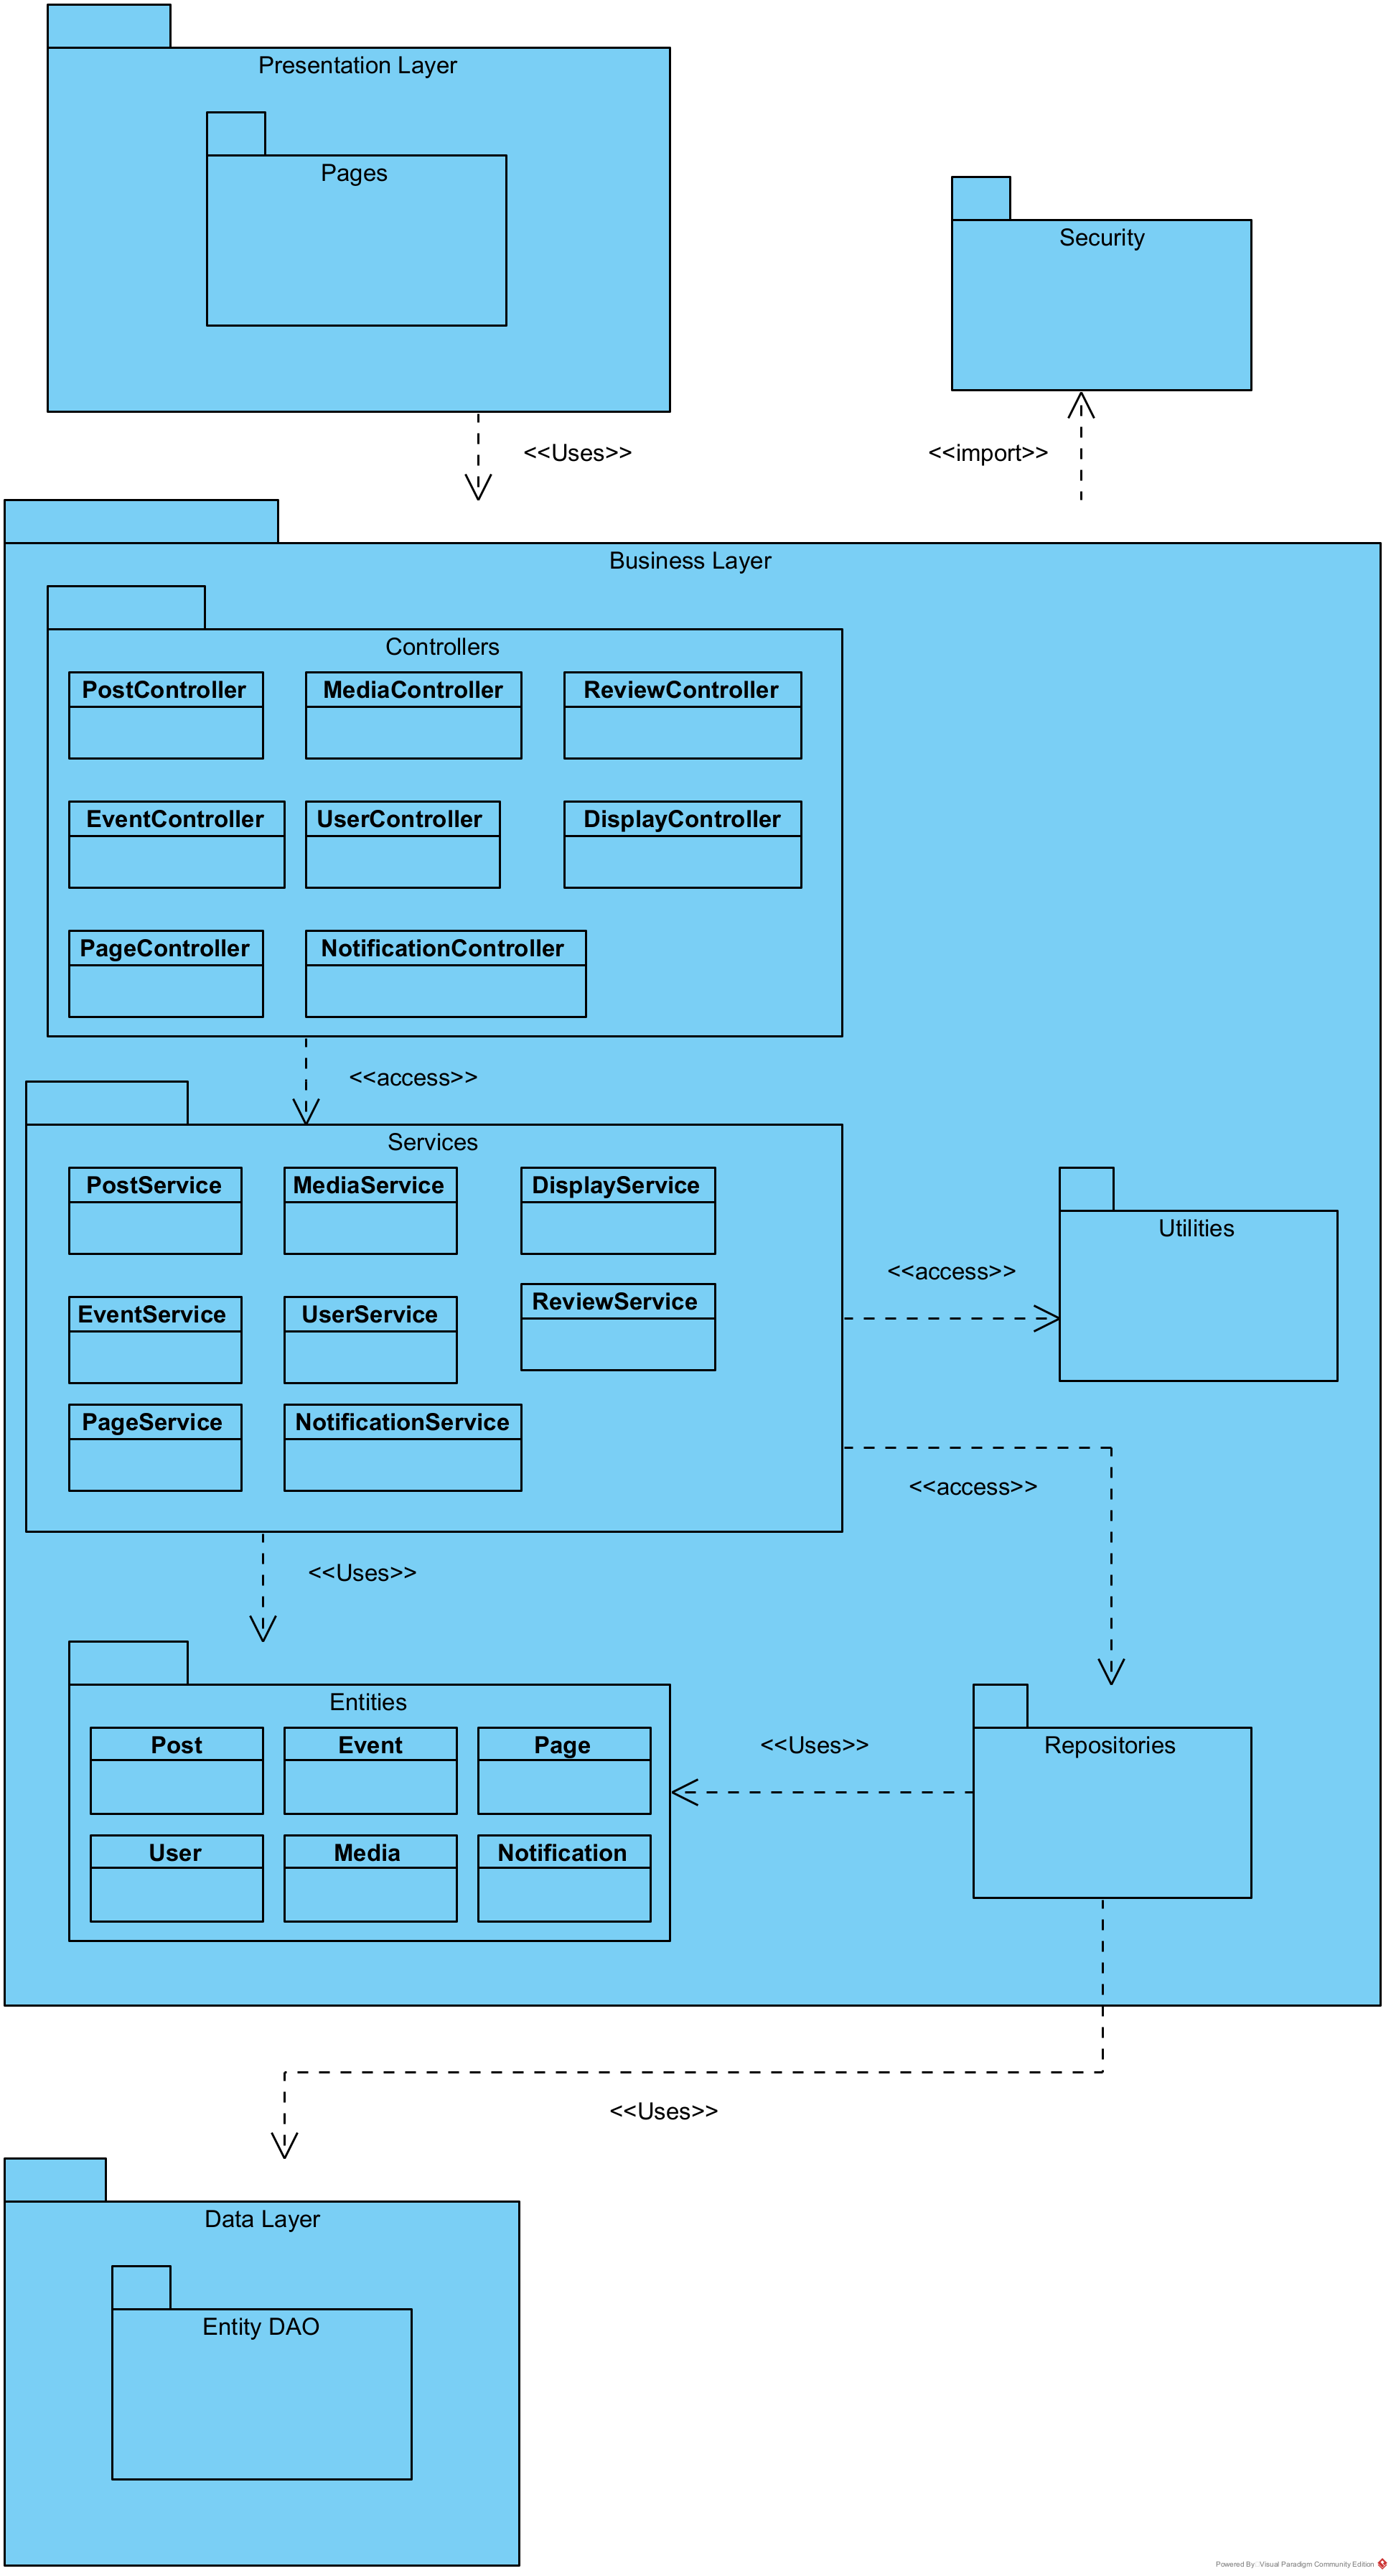
\includegraphics[width=.64\textwidth]{images/Package_Diagram.png}
    \centering
    \caption{Package Diagram}
\end{figure}

\section{Deployment Diagram}

\begin{figure}[H]
    \centering
    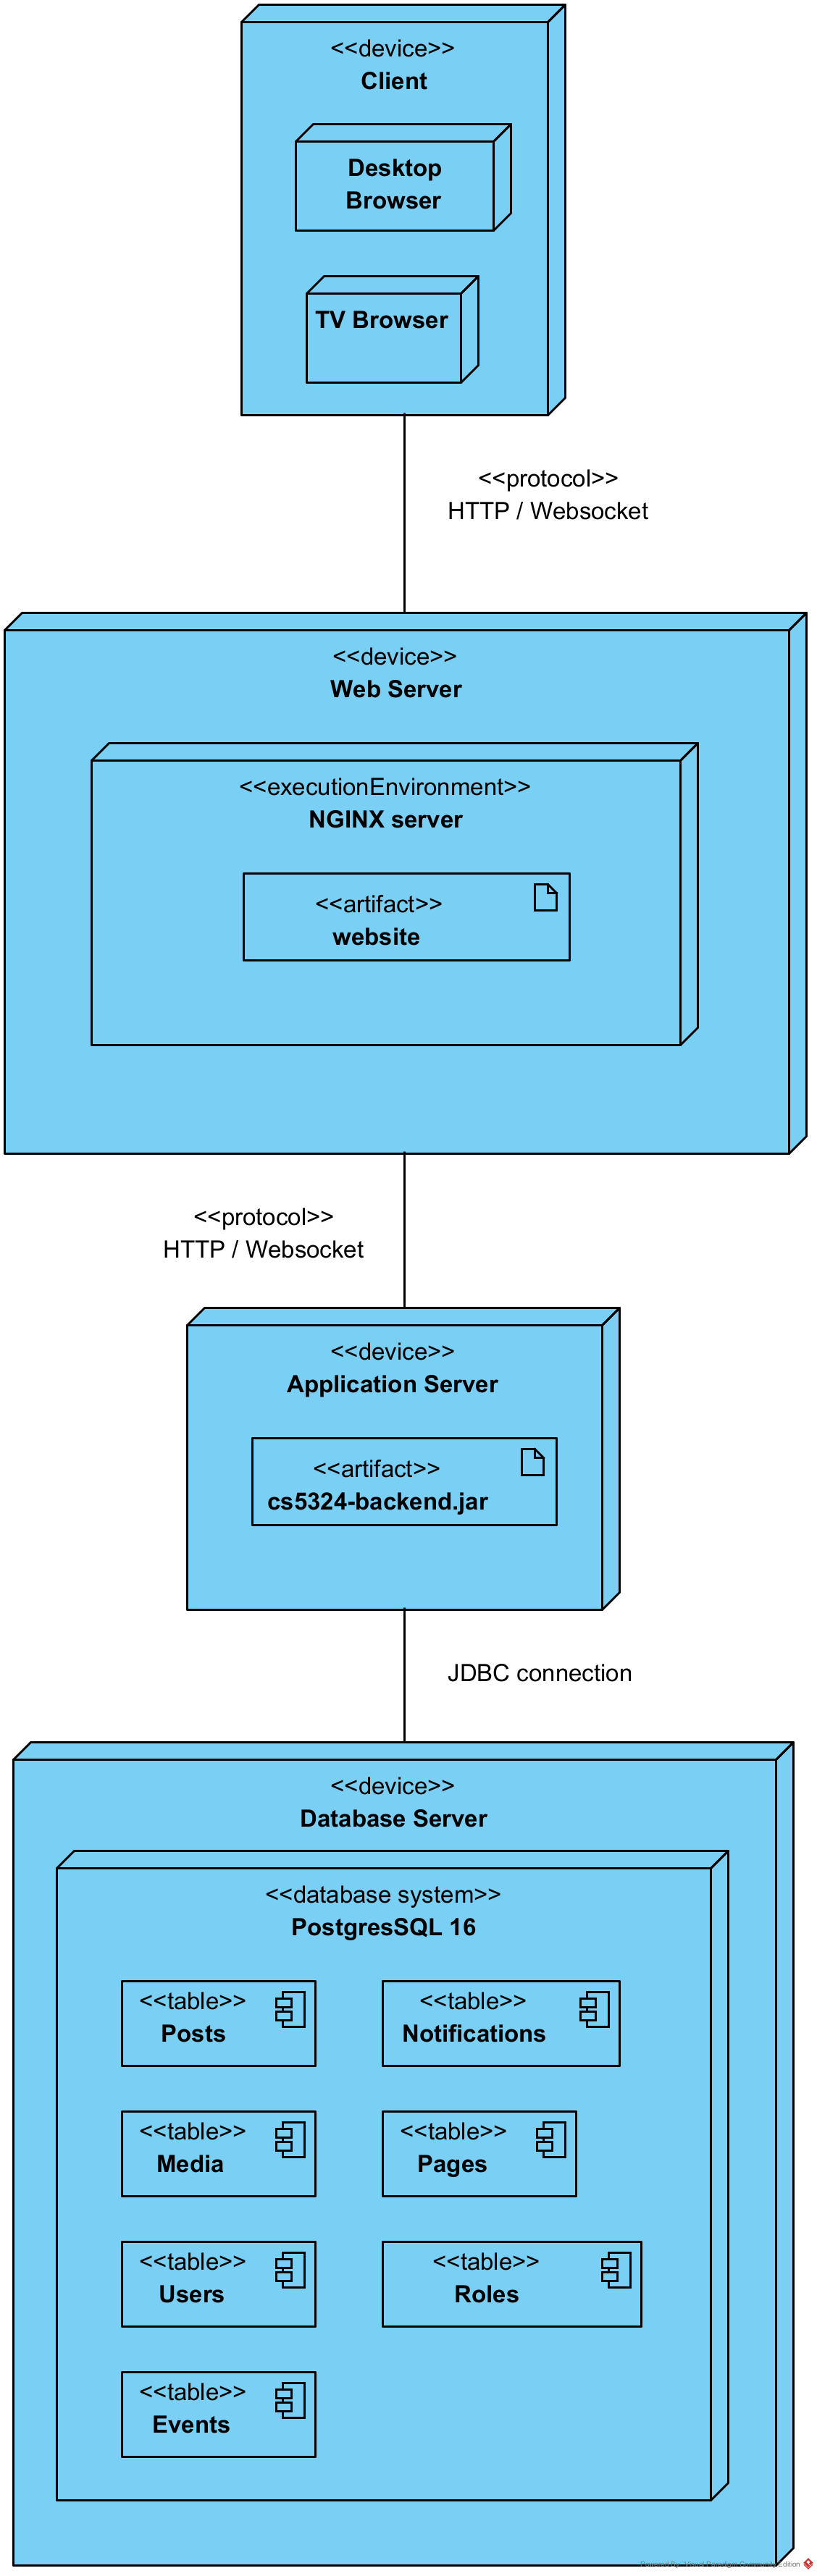
\includegraphics[width=.38\textwidth]{images/Deployment_Diagram.png}
    \centering
    \caption{Deployment Diagram}
\end{figure}

\end{document}